\section{Processi di Supporto}
\subsection{Documentazione}
	\subsubsection{Scopo}
	Ogni processo e attività significativi volti allo sviluppo del progetto sono documentati. Lo scopo di questa sezione è definire gli standard che riguardano i documenti prodotti durante il ciclo di vita del software.
	I documenti sono consultabili nelle apposite sezioni della repository\glo:\\ \url{https://github.com/8LabSolutions/Soldino}. 		
	\subsubsection{Aspettative}
	Le aspettative su questo processo riguardano:
	\begin{itemize}
		\item un'idea precisa relativa alla struttura della documentazione che deve essere prodotta durante il ciclo di vita del software;
		\item l'individuazione di una serie di norme per la stesura di documenti coerenti e validi.
	\end{itemize}
	\subsubsection{Descrizione}
	Questo capitolo contiene le decisioni e le norme che sono state scelte per la
	stesura, verifica e approvazione della documentazione ufficiale.  Tali norme  sono  tassative  per  tutti  i  documenti  formali.
	\subsubsection{Ciclo di vita del documento}
	Ogni documento segue le fasi del seguente ciclo di vita:
	\begin{itemize}
		\item \textbf{Creazione del documento}: il documento viene creato, in conformità alle norme e adeguandosi a documenti precedenti dello stesso tipo.
		Viene usato un template reperibile dalla cartella "latex" della repository\glosp remota;
		\item \textbf{Creazione della struttura}: viene creato un registro delle modifiche, un indice che traccia gli argomenti trattati nel documento, e a seconda delle necessità, un indice relativo alle figure e uno relativo alle tabelle presenti nel documento;
		\item \textbf{Realizzazione}: il documento viene scritto progressivamente in modo incrementale;
		\item \textbf{In revisione}: ogni voce del documento è prodotta interamente, ma è soggetta a verifiche per correggere, ampliare, semplificare quanto presente. La verifica di un frammento è svolta da almeno una persona, diversa da quella che ha scritto quel frammento;
		\item \textbf{Approvato}: il responsabile di progetto sancisce che il documento è stato completato, ed è quindi pronto per il rilascio.
	\end{itemize}

	\subsubsection{Template}
	Il gruppo ha creato un template \LaTeX{} per uniformare velocemente la struttura grafica e lo stile di formattazione dei documenti, in modo che i membri del team possano concentrarsi maggiormente, nella stesura del contenuto degli stessi. Lo scopo dei template è quello di permettere, a colui che redige il documento, di adottare automaticamente le conformità previste dalle \textit{Norme di Progetto}. Permette inoltre di agevolare la procedura di adeguamento alle nuove norme per la redazione, nel caso esse cambiassero.
	\subsubsection{Struttura dei documenti}
	Un file "main.tex" (il cui termine "main" verrà sostituito dal nome del documento) raccoglie tramite comandi di input le sezioni di cui è composto il documento. Tra i file in input ci sono:
	\begin{itemize}
		\item "package.tex", che contiene i pacchetti necessari alla compilazione;
		\item "config.tex", contenente comandi \LaTeX{} creati dal team.
	\end{itemize}
		\paragraph{Prima pagina} \mbox{}\\ \mbox{}\\
		Il frontespizio è la prima pagina del documento ed è così strutturata:
		\begin{itemize}
			\item \textbf{Logo del gruppo}: logo di \textit{8Lab Solutions} visibile come primo elemento centrato orizzontalmente in alto;
			\item \textbf{Gruppo e progetto}: nome del gruppo e del progetto \textit{Soldino}, visibile centralmente subito sotto il logo;
			\item \textbf{Titolo}: nome del documento, posizionato centralmente in grassetto;
			\item \textbf{Tabella}: presente sotto il titolo del documento, centrale e contenente le seguenti informazioni:
			\begin{itemize}
				\item \textbf{Versione}: versione del documento;
				\item \textbf{Approvazione}: nome e cognome dei membri del gruppo incaricati dell'approvazione del documento;
				\item \textbf{Redazione}: nome e cognome dei membri del gruppo incaricati della redazione del documento;
				\item \textbf{Verifica}: nome e cognome dei membri del gruppo incaricati della verifica del documento;
				\item \textbf{Stato}: stadio corrente del ciclo di vita del documento;
				\item \textbf{Uso}: tipo d'uso che può essere "interno" o "esterno";
				\item \textbf{Destinato a}: destinatari del documento.
			\end{itemize}
			\item \textbf{Descrizione}: descrizione sintetica relativa al documento, centrale, posta sotto la tabella descrittiva;
			\item \textbf{Recapito}: indirizzo di posta elettronica del gruppo, posizionato centralmente in fondo alla pagina.
		\end{itemize}
		\paragraph{Registro modifiche} \mbox{}\\ \mbox{}\\
		Ogni documento dispone di un changelog\glo: una tabella posta a seguito della prima pagina che contiene le modifiche apportate al documento. Nel changelog\glo sono indicati:
		\begin{itemize}
			\item versione del documento dopo la modifica;
			\item data della modifica;
			\item nominativo di chi ha modificato;
			\item ruolo di chi ha modificato;
			\item descrizione sintetica della modifica.
		\end{itemize}
		\paragraph{Indice} \mbox{}\\ \mbox{}\\
		Gli indici hanno lo scopo di riepilogare e dare una visione macroscopica della struttura del documento, mostrando le parti gerarchiche di cui è composto.\newline 
		Ogni documento è corredato dall'indice dei contenuti, posizionato dopo il changelog\glo. Se sono presenti tabelle o immagini all'interno del documento, l'indice dei contenuti è seguito prima dalla lista delle figure, poi dalla lista delle tabelle.
		\paragraph{Contenuto principale} \mbox{}\\ \mbox{}\\
		La struttura delle pagine di contenuto è così strutturata:
		\begin{itemize}
			\item in alto a sinistra è presente il logo del gruppo;
			\item in alto a destra è riportato il nome del documento;
			\item una riga divide l'intestazione dal contenuto;
			\item il contenuto della pagina è posto tra l'intestazione e il piè di pagina;
			\item una riga divide il contenuto dal piè pagina;
			\item in basso a destra è posto il numero della pagina corrente.
		\end{itemize}
		\paragraph{Verbali} \mbox{}\\ \mbox{}\\
		I verbali vengono prodotti dal/i soggetto/i incaricato/i alla loro stesura in occasione di incontri tra i membri del team con o senza la presenza di esterni. Per i verbali è prevista un'unica stesura. Tale	scelta è motivata dal fatto che apportare modifiche implica una modifica delle decisioni prese in modo retroattivo.
		I verbali seguono la struttura degli altri documenti, ma il corpo del verbale è suddiviso in introduzione e contenuto.
		L'introduzione contiene:
		\begin{itemize}
			\item \textbf{Luogo}: luogo di svolgimento dell'incontro;
			\item \textbf{Data}: data dell'incontro(in formato YYYY-MM-DD);
			\item \textbf{Ora di inizio}: l'orario di inizio dell'incontro;
			\item \textbf{Ora di fine}: l'orario di fine dell'incontro;
			\item \textbf{Partecipanti}: l'elenco dei membri del gruppo che erano presenti all'incontro e, se presenti, i nominativi di persone esterne al gruppo che hanno partecipato. Un esempio, sono i nomi dei componenti di \textit{Red Babel}, a fianco al quale deve essere indicato "(proponente)";
			\item \textbf{Argomenti affrontati}: ciò di cui si è discusso durante l'incontro in forma riassuntiva e facendo risaltare gli argomenti principali.
		\end{itemize}
	Il contenuto è composto da:
	\begin{itemize}
		\item una descrizione più approfondita in merito agli argomenti trattati durante l'incontro;
		\item un riepilogo dei tracciamenti in forma tabellare che elenca le decisioni emerse: assegna ad ognuna di loro un codice e le descrive. Sarà ripresa successivamente.
	\end{itemize}
		Ogni \textit{Verbale} dovrà essere denominato secondo il seguente formato: \newline \newline
		\centerline{\textbf{TipologiaYYYY-MM-DD}} \newline \newline
		dove per "Tipologia" si intende il tipo di verbale:
		\begin{itemize}
			\item \textbf{Interno}: concentrato sul riassunto dell'incontro dei membri del team;
			\item \textbf{Esterno}: concentrato sulla trattazione di argomenti con partecipanti esterni al gruppo, in particolare domande e risposte riguardanti il progetto in sè.
		\end{itemize}
		La sezione "Riepilogo tracciamenti" avrà la funzione di tenere traccia delle decisioni emerse da ogni incontro, sotto forma di tabella riassuntiva a fine di ogni verbale. Il formalismo utilizzato dalla tabella dovrà essere il seguente: \newline \newline
		\centerline{\textbf{Tipologia\_X.Y}} \newline \newline
		Dove:
		\begin{itemize}
			\item per "Tipologia" basterà indicare l'iniziale della tipologia del verbale(I=Interno/E=Esterno);
			\item "X.Y": X si riferisce al numero dell'incontro mentre per Y si intende il numero progressivo della decisione presa dal gruppo(partendo da 1).
		\end{itemize}	
		\paragraph{Note a piè di pagina} \mbox{}\\ \mbox{}\\
		In caso di presenza di note da esplicare, esse vanno indicate nella pagina corrente, in basso a sinistra. Ogni nota deve riportare un numero e una descrizione.		
	\subsubsection{Norme tipografiche}
		\paragraph{Convenzioni sui nomi dei file} \mbox{}\\ \mbox{}\\
		I nomi di file (estensione esclusa) e cartelle utilizzano la convenzione "Snake case\glo" e alcune regole aggiuntive elencate di seguito:
		\begin{enumerate}
			\item i nomi dei file composti da più parole usano il carattere underscore come carattere separatore;
			\item i nomi sono scritti interamente in minuscolo;
			\item le preposizioni non si omettono.
		\end{enumerate}
		Alcuni esempi \textbf{corretti} sono:
		\begin{itemize}
			\item studio\_di\_fattibilità;
			\item analisi\_dei\_requisiti.
		\end{itemize}	 	
		Alcuni esempi \textbf{non corretti} sono: 
		\begin{itemize}
			\item Norme\_di\_progetto (usa maiuscole);
			\item norme-di-progetto (carattere separatore errato);
			\item norme\_progetto (omette "di").
		\end{itemize}
		\paragraph{Glossario}
		\begin{itemize}
			\item ogni termine del \textit{Glossario} è marcato con una \textbf{G} maiuscola a pedice in ogni sua occorrenza;
			\item se la voce è presente ripetutamente nello stesso paragrafo non è necessario marcarla in ogni sua occorrenza, ma è possibile indicare la \textbf{G} a pedice solo nella prima occorrenza;
			\item se nel \textit{Glossario v1.0.0} un termina presenta una descrizione che utilizza termini da glossario, è necessario trattare questi termini come tali, segnando la \textbf{G} a pedice e aggiungendoli al documento con la relativa descrizione;
			\item non vengono segnate con la \textbf{G} a pedice  le parole da \textit{Glossario} presenti nei titoli e nelle didascalie di immagini e tabelle.
		\end{itemize}			
		\paragraph{Stile del testo}
		\begin{itemize}
			\item \textbf{Grassetto}:
			viene applicato se necessario alle voci di un elenco puntato, a titoli o a termini di frasi su cui si vuol far ricadere l'attenzione del lettore;
			\item \textbf{Corsivo}: vengono scritti in corsivo il nome del progetto \textit{Soldino}, il nome del gruppo \textit{8Lab Solutions} ed il nome del gruppo dei proponenti, ovvero \textit{Red Babel}; %token\glosp coniato nella piattaforma,  \textit{Cubit};
			\item \textbf{Maiuscolo}: vengono scritti con sole lettere maiuscole tutti gli acronimi. Nel caso di nomi o titoli composti da più parole verrà indicato con la lettera maiuscola solamente la prima lettera della prima parola, lasciando in minuscolo il restante (esclusi nomi dei documenti che sono normati secondo quanto segue);
			\item \textbf{Nomi dei documenti}:
			\begin{itemize}
				\item ogni volta che si cita un documento, si deve indicare con la lettera maiuscola le iniziali dei nomi di cui è composto (\textit{e.g.} Analisi dei Requisiti), ma senza specificare la versione, riportando il tutto in corsivo;
				\item quando si fa riferimento al documento vero e proprio o a qualcosa in esso contenuto si segue la prima convenzione ma si aggiunge la versione del documento v*.0.0 (separata da uno spazio), anch'essa in corsivo;
				\item ogni volta che si utilizza il documento come titolo o in una voce di elenco seguita da una descrizione, si deve seguire la prima convenzione ma senza utilizzare il corsivo.
			\end{itemize}
		\end{itemize}
		\paragraph{Elenchi puntati} \mbox{}\\ \mbox{}\\
		Ogni voce di un elenco comincia per lettera \textbf{minuscola}, a patto che non subentrino altre norme, e termina per \textbf{";"}, eccetto l'ultima che termina per \textbf{"."}. I sottoelenchi innestati dentro una voce di elenco, rispettano le medesime regole, poiché la loro funzione è analoga.\newline
		Se le voci dell'elenco sono della forma \textit{termine - descrizione}, si pongono i termini in grassetto.
		\paragraph{Formati comuni} \mbox{}\\ \mbox{}\\
		In conformità allo standard ISO 8601, le date devono essere scritte secondo il formato: \newline \newline
		\centerline{YYYY-MM-DD}
		\begin{itemize}
			\item \textbf{YYYY}: rappresentazione dell'anno con quattro (4) cifre;
			\item\textbf{MM}: rappresentazione del mese con due (2) cifre;
			\item \textbf{DD}: rappresentazione del giorno con due (2) cifre.			
		\end{itemize}
		\paragraph{Sigle} \mbox{}\\ \mbox{}\\
		Il progetto prevede la redazione di un insieme di documenti, suddivisi in documenti interni e documenti esterni. Essi sono elencati di seguito con le rispettive sigle.\newline
		I documenti esterni sono:	
		\begin{itemize}
			\item \textbf{Analisi dei Requisiti - AdR}: stabilisce le caratteristiche che il software deve rispettare;
			\item \textbf{Manuale Utente - MU}: ad uso degli utilizzatori del software;
			\item \textbf{Manuale Sviluppatore - MS}: per gli sviluppatori e manutentori;
			\item \textbf{Piano di Progetto - PdP}:  concerne la gestione del progetto, evidenziandone la fattibilità e le criticità; tratta di tempi, costi, obiettivi, rischi, vincoli;
			\item \textbf{Piano di Qualifica - PdQ}: : descrive la qualità del software e dei processi, e come la si intende raggiungere mediante l'uso di strumenti, metriche e processi stessi.
		\end{itemize}
		I documenti interni sono:
		\begin{itemize}
			\item \textbf{Glossario - G}: raccoglie i termini di interesse per il team di sviluppo e sui quali è necessaria una descrizione che ne chiarisca il significato;
			\item \textbf{Norme di Progetto - NdP}: sono un riferimento normativo per lo svolgimento delle attività di progetto;
			\item \textbf{Studio di Fattibilità - SdF}: descrive sommariamente i capitolati e spiega la loro scelta o esclusione.
		\end{itemize}
		Un caso particolare di documenti, sono i verbali, che possono essere esterni o interni:
		\begin{itemize}
			\item \textbf{Verbale - V}: descrive le interazioni avvenute durante un incontro con il proponente (verbale esterno) o tra i membri del team (verbale interno); sono orientati a dare informazioni semplici, di veloce lettura e complete.
		\end{itemize}
		Le diverse fasi del progetto sono le seguenti, accompagnate dalle relative sigle:
		\begin{itemize}
			\item \textbf{Revisione dei Requisiti - RR}: studio iniziale del capitolato\glo, se ben fatto permette al gruppo di aggiudicarselo;
			\item \textbf{Revisione di Progettazione - RP}: riguarda la definizione dell'architettura del software e di una Proof of Concept\glosp per mostrare la fattibilità;
			\item \textbf{Revisione di Qualifica - RQ}: riguarda la definizione dettagliata e la codifica del prodotto;
			\item \textbf{Revisione di Accettazione - RA}: se il prodotto soddisfa i requisiti del proponente, viene accettato e rilasciato.		
		\end{itemize}	
		Altre sigle presenti nei documenti interessano i ruoli assunti dai componenti del team:
		\begin{itemize}
			\item \textbf{responsabile di progetto - Re};
			\item \textbf{amministratore - Ad};
			\item \textbf{analista - An};
			\item \textbf{progettista - Pt};
			\item \textbf{programmatore - Pr};
			\item \textbf{verificatore - Ve};
		\end{itemize}
		\subsubsection{Elementi grafici}
		\paragraph{Tabelle} \mbox{}\\ \mbox{}\\
		In tutti i documenti \LaTeX{} le tabelle sono scritte allo stesso modo: fare riferimento alla Wiki su GitHub per i comandi necessari.\newline 
		Ogni tabella deve essere accompagnata dalla propria didascalia descrittiva, la "caption", da posizionare subito sopra la tabella a cui si riferisce. \'E stata scelta questa convenzione per adattarsi agli standard usati dalla maggioranza della community di \LaTeX{}; nella didascalia deve comparire il numero della sezione a cui si riferisce, seguita in modo incrementale dal numero progressivo delle tabelle di quella sezione.
		\begin{itemize}
			\item \textbf{{X.Y}}: rappresenta la sezione;
			\item \textbf{{Z}}: rappresenta il numero progressivo della tabella nella sezione.
		\end{itemize}
		Fanno eccezione le tabelle dei changelog\glosp che non hanno didascalia e le tabelle dei casi d'uso presenti nel documento \textit{Analisi dei Requisiti}.
		\paragraph{Immagini} \mbox{}\\ \mbox{}\\
		Le immagini sono centrate e hanno una didascalia descrittiva. 
		\paragraph{Diagrammi UML} \mbox{}\\ \mbox{}\\
		Tutti i diagrammi UML\glosp vengono inseriti nei documenti sotto forma di immagine.
	\subsubsection{Strumenti}
		\paragraph{\LaTeX} \mbox{}\\ \mbox{}\\
		Lo strumento scelto per la scrittura di documenti è \LaTeX{}, un linguaggio basato sul programma di composizione tipografica \TeX{} che permette di scrivere documenti in modo ordinato, modulare, collaborativo e scalabile.
		\paragraph{\TeX{}studio} \mbox{}\\ \mbox{}\\
		Per la stesura del codice \LaTeX{} è stato utilizzato l'editor \TeX{}studio. Questo strumento, oltre ad integrare un compilatore e un visualizzatore PDF, fornisce suggerimenti di completamento per comandi \LaTeX{}. \newline
		\centerline{\url{https://www.texstudio.org/}}
		\begin{figure}[H]
			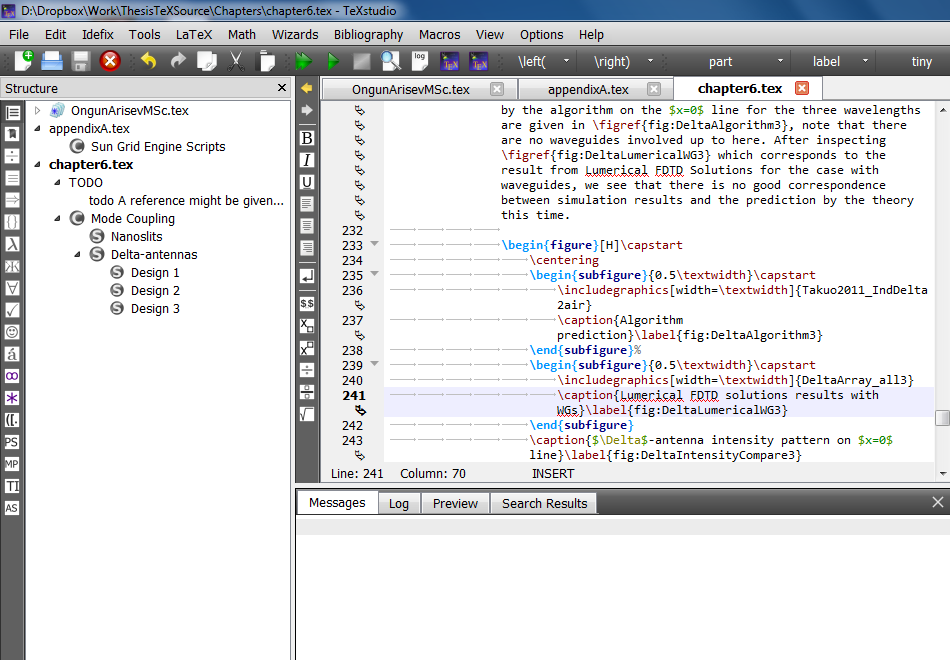
\includegraphics[width=0.99\linewidth]{res/images/latex.jpg}
			\caption{\TeX{}studio - per la stesura dei documenti}
		\end{figure} 
		\paragraph{Draw.io} \mbox{}\\ \mbox{}\\
		Draw.io, già citato in precedenza, viene utilizzato per la produzione degli UML\glo. \newline
		\centerline{\url{https://www.draw.io/}}
		
	\subsection{Gestione della configurazione}
	\subsubsection{Scopo}
	Lo scopo della configurazione è di creare ordine tra software e documenti. Tutto ciò che è configurato si trova in un posto preciso, ha uno stato identificativo, è modificato secondo procedure e posto sotto versionamento.
	\subsubsection{Versionamento}
	\paragraph{Codice di versione del documento} \mbox{}\\ \mbox{}\\
	Ogni documento, deve avere una storia, ricostruibile attraverso le sue versioni. Ogni versione deve corrispondere a una riga della tabella delle modifiche. Ogni numero di versione è composto da tre cifre:
	\begin{center}
		X.Y.Z
	\end{center}
	\begin{itemize}
		\item \textbf{X}: rappresenta una versione stabile del documento, resa tale dopo l' approvazione del responsabile di progetto:
		\begin{itemize}
			\item inizia da 0;
			\item viene incrementato dal responsabile di progetto all'approvazione del documento.
		\end{itemize}
		\item \textbf{Y}: rappresenta una versione parzialmente stabile del documento che è stata soggetta a verifica da parte di un verificatore:
		\begin{itemize}
			\item inizia da 0;
			\item viene incrementato dal verificatore ad ogni verifica;
			\item quando viene incrementato X, viene riportato a 0.
		\end{itemize}
		\item \textbf{Z}: rappresenta una versione instabile del documento in fase di lavorazione da parte dei redattori:
		\begin{itemize}
			\item inizia da 0;
			\item viene incrementato dal redattore del documento ad ogni modifica;
			\item quando viene incrementato Y, viene riportato a 0.
		\end{itemize}			
	\end{itemize}
	\paragraph{Tecnologie} \mbox{}\\ \mbox{}\\
	Per le parti del progetto da versionare si è scelto di usare il sistema di versionamento distribuito Git, usando il servizio di GitHub per ospitare la repository\glosp remota.
	\paragraph{Repository} \mbox{}\\ \mbox{}\\
	I membri del team possono interagire con il VCS (Version Control System) sia da linea di comando, sia attraverso software che ne migliorano l'usabilità, come GitFlow e GitKraken. La versione comune e ufficiale del progetto è ospitata in una repository\glosp remota su Github all'indirizzo: \newline \newline
	\centerline{\url{https://github.com/8LabSolutions/Soldino}}
	\paragraph{Struttura del repository} \mbox{}\\ \mbox{}\\
	Ci sono due tipi di repository\glo{}, la cui struttura è identica:
	\begin{itemize}
		\item \textbf{locale}: ogni membro del gruppo lavora sui file clonati dal repository\glo{} remoto nel proprio computer;
		\item \textbf{remoto}: pubblicato su GitHub, contiene il lavoro svolto da ogni componente e che viene condiviso con il team.
	\end{itemize}						
	Entrambe i tipi di repository\glosp sono organizzati in cartelle:
	\begin{itemize}
		\item \textbf{latex}: contiene tutti i file che definiscono il template \LaTeX{} per la creazione di un nuovo documento. Tra questi vi sono i file che definiscono i comandi personalizzati utilizzati dal gruppo e i package che devono essere inclusi per poter compilare i documenti;
		\item \textbf{Guide}: cartella che contiene delle brevi guide di carattere pratico, come brevi spiegazioni per l'utilizzo dei comandi \LaTeX{} poco conosciuti;
		\item \textbf{RR}: raccoglie i file sorgenti per la compilazione dei documenti, suddivisi tra esterni ed interni, realizzati per la Revisione dei Requisiti;
		\item Saranno aggiunte in futuro cartelle distinte nominate \textbf{RP}, \textbf{RQ} e \textbf{RA} contenenti i file delle rispettive consegne.
	\end{itemize}
	La suddivisione dei file per revisione aiuta ad evidenziare il lavoro svolto per ogni consegna e migliora la tracciabilità dei file all'interno di ognuna di esse.
	\paragraph{Tipi di file e .gitignore} \mbox{}\\ \mbox{}\\
	I file utilizzati per la documentazione del progetto sono:
	\begin{itemize}
		\item file con estensione .tex di \LaTeX{};
		\item file con estensione .pdf che sono oggetto di consegna;
		\item alcuni file testuali e immagini di supporto ai precedenti.
	\end{itemize}			
	Il file ".gitignore" è presente al livello più esterno della repository\glosp ed elenca tutti i file da escludere dal versionamento. 
	\paragraph{Utilizzo di Git} \mbox{}\\ \mbox{}\\
	Il repository\glosp di Git è composto da vari branch, per lavorare in modo modulare e collaborativo.  
	Quindi viene consiglia questa procedura:
	\begin{enumerate}
		\item scegliere il branch su cui si vuole lavorare in base al compito assegnato;
		\item eseguire il pull dal repository\glosp remoto che effettua l'aggiornamento del proprio repository\glosp locale;
		\item svolgere il lavoro assegnato, che può consiste nell'aggiunta di nuovo materiale o nella modifica di file già presenti;
		\item eseguire il comando di aggiunta dei file nuovi o modificati da condividere all'area di staging\glo;
		\item eseguire il comando di commit dei file aggiunti, corredato da un messaggio che identifica il task eseguito;
		\item eseguire il push del commit sul repository\glosp remoto.
	\end{enumerate}
	\paragraph{Gestione delle modifiche} \mbox{}\\ \mbox{}\\
	Tutti i membri del team possono modificare i file in ogni branch, ad eccezione di quelli presenti nel branch master, per il quale occorre fare una pull request\glosp e ottenere l'approvazione di un altro membro .\newline
	Per effettuare modifiche maggiori sui contenuti o sulla struttura dei file è previsto di:
	\begin{itemize}
		\item contattare il responsabile del file da modificare;
		\item suggerire la modifica da effettuare;
		\item se il responsabile valuta positivamente la modifica, allora la applica.
	\end{itemize}
	Per modifiche minori, come correzioni grammaticali o miglioramenti sintattici, si consiglia di modificare indipendentemente.\newline
	In ambo i casi è opportuno commentare i propri commit con chiarezza per risalire facilmente alle modifiche.

\subsection{Gestione della Qualità}
	\subsubsection{Scopo}
	Lo scopo è di garantire che il prodotto e i servizi offerti rispettino gli obiettivi di qualità e che i bisogni del proponente siano soddisfatti.
	\subsubsection{Aspettative}
	Attraverso la gestione della qualità si intende ottenere:
	\begin{itemize}
		\item qualità nell'organizzazione e nei suoi processi;
		\item qualità nel prodotto;
		\item qualità provata oggettivamente;
		\item soddisfazione finale di cliente e proponente.
	\end{itemize}
	\subsubsection{Descrizione}
	Per la trattazione approfondita della gestione della qualità si fa riferimento al \textit{Piano di Qualifica v1.0.0}, dove sono descritte le modalità utilizzate per garantire la qualità nello sviluppo del progetto. In particolare, in tale documento:
	\begin{itemize}
		\item sono presentati gli standard utilizzati;
		\item sono individuati i processi di interesse negli standard;
		\item sono individuati gli attributi del software più significativi per il progetto.
	\end{itemize}
	Per ogni processo vengono descritti:
	\begin{itemize}
		\item gli obiettivi da perseguire;
		\item le strategie da applicare;
		\item le metriche da utilizzare.
	\end{itemize}
	L'obiettivo è quello di controllare e migliorare i processi e i loro risultati.
	Per ogni prodotto vengono associati:
	\begin{itemize}
		\item gli obiettivi da perseguire;
		\item le metriche da utilizzare.
	\end{itemize}
	In questo caso si mira ad ottenere software e documentazione di qualità soddisfacente.
	\subsubsection{Attività}
	Le tre attività principali del processo sono:
	\begin{itemize}
		\item \textbf{Pianificazione}: porsi degli obiettivi di qualità, definire strategie per raggiungerli e disporre di conseguenza le persone e le risorse nel modo migliore;
		\item \textbf{Valutazione}: mettere in atto la pianificazione, applicando i criteri, misurando e monitorando i risultati; 
		\item \textbf{Reazione}: sulla base dei risultati, adattare le proprie strategie, criteri e piani.
	\end{itemize}
	\subsubsection{Strumenti}
	Gli strumenti predefiniti per la qualità sono: 
	\begin{itemize}
		\item forniti dallo standard \textbf{ISO-12207};
		\item le metriche.
	\end{itemize} 
		
\subsection{Verifica}
	\subsubsection{Scopo}
	Il processo di verifica ha per scopo la realizzazione di prodotti corretti, coesi e completi. Sono soggetti a verifica il software e i documenti. 
	\subsubsection{Aspettative}
	Il corretto svolgimento del processo di verifica rispetta i punti seguenti:	
	\begin{itemize}
		\item viene effettuata seguendo procedure definite;
		\item vi sono criteri chiari e affidabili da seguire per verificare;
		\item i prodotti passano attraverso fasi successive, ognuna delle quali è verificata;
		\item dopo la verifica il prodotto è in uno stato stabile;
		\item rende possibile la validazione.
	\end{itemize}
	\subsubsection{Descrizione}
	Il processo di verifica prende in input ciò che è già stato prodotto e lo restituisce in uno stato conforme alle aspettative. Per ottenere tale risultato ci si affida a processi di analisi e test.
	\subsubsection{Attività}
		\paragraph{Analisi} \mbox{}\\ \mbox{}\\
		Il processo di analisi si suddivide in statica e dinamica. \newline \newline
			\textbf{Analisi statica} \mbox{}\\ \mbox{}\\
			L'analisi statica effettua controlli su documenti e codice, di cui valuta e applica la correttezza (intesa come assenza di errori e difetti), la conformità a regole e la coesione\glosp dei componenti.\newline Per effettuare analisi statica esistono metodi manuali di lettura (attuati da persone) e metodi formali (attuati da macchine). Quelli manuali sono due:
			\begin{itemize}
				\item \textbf{Walkthrough}: i vari componenti del team analizzano gli oggetti nella loro totalità per cercare anomalie, senza sapere inizialmente se vi siano difetti, quali e dove siano;
				\item \textbf{Inspection}: i verificatori usano liste di controllo per fare ispezione cercando errori specifici in parti specifiche.
			\end{itemize}
			A seguire sono descritte le liste di controllo utilizzabili per le ispezioni. Si prevede l'ampliamento delle viste al progredire delle stesse ispezioni e degli errori trovati.
%\begin{comment}
			\begin{table}[H]
				\centering\renewcommand{\arraystretch}{1.5}
				\arrayrulecolor{white}
				\caption{Errori frequenti nei documenti}
				\begin{tabular}{c|c}
					
					\rowcolorhead
					{\colorhead \textbf{Oggetto}} &
					{\colorhead \textbf{Controllo} }\\
					
					\rowcolorlight
					{\colorbody Formato data} & {\colorbody Deve seguire il formato americano \textit{YYYY-MM-DD}} 
					\\
					
					\rowcolordark
					{\colorbody Sintassi} & {\colorbody  La frase è troppo complessa e può essere semplificata } 
					\\	
					
					\rowcolorlight
					{\colorbody Parte mancante} & {\colorbody Controllare titoli vuoti o sezioni di grandezza insolita} 
					\\
					
					\rowcolordark
					{\colorbody Forma dei verbi} & {\colorbody In generale è preferibile il presente indicativo} 
					\\
					
					\rowcolorlight
					{\colorbody Punteggiatura degli elenchi} & {\colorbody Ogni voce termina in \textbf{";"} eccetto l'ultima che termina in \textbf{"."}} 
					\\
				\end{tabular}
			\end{table}
%\end{comment}
			% PLACEHOLDER: lista di ispezione del codice, da aggiungere quando si fa il codice.				
			\mbox{}\\								
			\textbf{Analisi dinamica} \mbox{}\\ \mbox{}\\
			L'analisi dinamica è una tecnica di analisi del prodotto software che richiede la sua esecuzione. Viene effettuata  mediante dei test che verificano se il prodotto funziona e se ci sono anomalie. 
			
		\paragraph{Test} \mbox{}\\ \mbox{}\\
		I test sono l'attività fondamentale dell'analisi dinamica: il loro scopo è verificare che il codice scritto funzioni correttamente.
		Per ogni test devono essere definiti i seguenti parametri:
		\begin{itemize}
			\item \textbf{ambiente}: sistema hardware e software sul quale verrà eseguito il test;
			\item \textbf{stato iniziale}: lo stato iniziale dal quale il test viene eseguito;
			\item \textbf{input}: input inserito;
			\item \textbf{output}: output atteso;
			\item \textbf{istruzioni aggiuntive}: ulteriori istruzioni su come va eseguito il test e su come vanno interpretati i risultati ottenuti.
		\end{itemize}
		Test ben scritti devono:
		\begin{itemize}
			\item essere ripetibili;
			\item specificare l'ambiente di esecuzione;
			\item identificare input e output richiesti;
			\item avvertire di possibili effetti indesiderati;
			\item fornire informazioni sui risultati dell'esecuzione in forma di file di log.
		\end{itemize}	
			
		\noindent{Ci sono vari tipi di test del software, ognuno dei quali ha un diverso oggetto di verifica e scopo.} \newline \newline
			\textbf{Test di unità} \mbox{}\\ \mbox{}\\
			I test di unità si eseguono su unità di software. Questi test si concentrano sul funzionamento delle unità individuali. Dati gli input possibili in un unità, si suddividono gli input in partizioni di equivalenza e si prova se gli input attesi danno gli output previsti. Le singole unità possono essere testate con l'ausilio di driver\glosp e stub\glosp. \newline \newline
			\textbf{Test di integrazione} \mbox{}\\ \mbox{}\\
			Dopo aver superato i test di unità, le stesse unità vengono assemblate in agglomerati progressivamente più grandi. Il test di integrazione si concentra sulle interfacce tra i componenti. Un agglomerato che supera il test di integrazione costituisce quindi una nuova unità per un agglomerato di grandezza maggiore. Questa procedura si ripete fino a raggiungere la dimensione totale del sistema. \newline \newline
			\textbf{Test di sistema} \mbox{}\\ \mbox{}\\
			Il sistema viene testato nella sua interezza, una volta integrati tutti i suoi componenti. Ci si concentra sulle interazioni tra le parti, sul comportamento emergente\glosp delle caratteristiche del sistema e sulla copertura\glosp di tutte le funzionalità. Questo tipo di test porta alla luce le ipotesi errate che i diversi sviluppatori fanno su parti del software sviluppate da altri.
			In questa fase ci si assicura che il sistema rispetti tutte le specifiche definite nell'\textit{Analisi dei Requisiti}. \newline \newline
			\textbf{Test di regressione} \mbox{}\\ \mbox{}\\
			Si effettua di seguito ad una modifica del sistema e consiste nella riesecuzione dei test esistenti: si combina bene con l'automazione dei test. \newline \newline
			\textbf{Test di accettazione} \mbox{}\\ \mbox{}\\
			Anche detto "test di collaudo", è simile al test di sistema per l'oggetto testato, ma viene eseguito con la collaborazione dei committenti. Si occupa di verificare il prodotto e, in particolare, il soddisfacimento del cliente. Il superamento del test di collaudo garantisce che il software sia pronto per essere rilasciato.
	\subsubsection{Strumenti}
		\paragraph{Verifica ortografica} \mbox{}\\ \mbox{}\\
		Viene utilizzata la verifica dell'ortografia in tempo reale, strumento integrato in \TeX{}studio che sottolinea in rosso le parole errate e in verde le ripetizioni a breve distanza secondo la lingua italiana.
		\paragraph{Validazione W3C} \mbox{}\\ \mbox{}\\
		Per la validazione delle pagine di markup HTML viene utilizzato lo strumento offerto dal W3C, raggiungibile al seguente indirizzo: \newline
		\centerline{\url{https://validator.w3.org/}} \newline \newline
		Per la validazione dei fogli di stile CSS viene utilizzato lo strumento offerto dal W3C, raggiungibile al seguente indirizzo: \newline
		\centerline{\url{https://jigsaw.w3.org/css-validator/}} \newline

		%\paragraph{Metriche} ????
		% da fare
\subsection{Validazione}
	\subsubsection{Scopo}
	Lo scopo della validazione è stabilire se il prodotto soddisfa il compito per cui è stato creato. Dopo la validazione, è garantito che il software rispetti i requisiti e che soddisfa i bisogni del committente.
	\begin{comment}
	\subsubsection{Aspettative}
	Una corretta implementazione di questo processo permette di individuare:
	\begin{itemize}
		\item una procedura di validazione;
		\item i criteri per la validazione del prodotto;
		\item le conformità del prodotto finito.
	\end{itemize}
	\end{comment}
	\subsubsection{Attività}
	Per validare il prodotto si devono rispettare i seguenti punti:
	\begin{itemize}
		\item identificare gli oggetti da validare;
		\item identificare una strategia con delle procedure di validazione in cui le procedure di verifica possono essere riutilizzare;
		\item applicare la strategia;
		\item valutare che i risultati rispettino le aspettative.
	\end{itemize}
